\documentclass[a4paper,fleqn]{cas-sc}

%Packages
\usepackage[authoryear,longnamesfirst]{natbib}
\usepackage[spanish]{babel}


%%%Author macros
\def\tsc#1{\csdef{#1}{\textsc{\lowercase{#1}}\xspace}}
\tsc{WGM}
\tsc{QE}
%%%

\newtheorem{theorem}{Theorem}
\newtheorem{lemma}[theorem]{Lemma}
\newdefinition{rmk}{Remark}
\newproof{pf}{Proof}
\newproof{pot}{Proof of Theorem \ref{thm}}



\begin{document}
\let\WriteBookmarks\relax
\def\floatpagepagefraction{1}
\def\textpagefraction{.001}

% Short title
\shorttitle{}    

% Short author
\shortauthors{Juan Alvarez, Christian Paredes}  

% Main title of the paper
\title[mode = title]{Análisis del desempeño histórico de las carteras recomendadas por varios bancos de inversión en función del perfil de riesgo de los clientes}  

% Title footnote mark
\tnotemark[1]

% Title footnote 1.
\tnotetext[1]{Trabajo de técnicas de investigación}

% First author
%
% Options: Use if required
% eg: \author[1,3]{Author Name}[type=editor,
%       style=chinese,
%       auid=000,
%       bioid=1,
%       prefix=Sir,
%       orcid=0000-0000-0000-0000,
%       facebook=<facebook id>,
%       twitter=<twitter id>,
%       linkedin=<linkedin id>,
%       gplus=<gplus id>]

\author[1]{Juan Fidel Alvarez Escontrela}%[
	%type=editor,
	%style=Español,
	%auid=001,
	%bioid=1,
	%prefix=Sir,
	%orcid=0000-0000-0000-0001,
	%twitter=www.twitter.com/juanfidelalvarez,
	%linkedin=www.linkedin.com/in/juanfidelalvarez,
	%gplus=001]
%]

% Corresponding author indication
%\cormark[1]

% Footnote of the first author
%\fnmark[]

% Email id of the first author
\ead{fidel220492@gmail.com}

% URL of the first author
\ead[url]{www.juanalvarez.com}

% Credit authorship
%\credit{Conceptualization of this study, Methodology, Software}

% Address/affiliation
\affiliation[1]{organization={Universidad de Santiago de Compostela},
            addressline={Campus Norte, Av. do Burgo das Nacións, s/n}, 
            city={Santiago de Compostela},
%          citysep={}, % Uncomment if no comma needed between city and postcode
            postcode={15782}, 
            %state={},
            country={España}}

% Second author
\author[2]{Christian L. Paredes Aguilera}%[
	%type=editor,
	%style=Espanol,
	%auid=002,
	%bioid=2,
	%prefix=Sir,
	%orcid=0009-0004-1216-9556,
	%twitter=www.twitter.com/christianparedes,
	%linkedin=www.linkedin.com/in/christianparedes,
	%gplus=002]
%]

\ead{soyfode@gmail.com}

\ead[url]{www.christianparedes.com}

\affiliation[2]{organization={Universidad de Vigo},
            addressline={R\'ua as Pedreiras, 2}, 
            city={Vigo},
%          citysep={}, % Uncomment if no comma needed between city and postcode
            postcode={36310}, 
            %state={},
            country={España}}

%\credit{Data curation, Writing - Original draft preparation}

% For a title note without a number/mark
%\nonumnote{}

% Here goes the abstract
\begin{abstract}
Este estudio se centra en analizar el desempeño histórico de las carteras recomendadas por los principales bancos de inversión a nivel internacional, considerando los perfiles de riesgo de sus clientes y la estrategia de inversión utilizada (activa o pasiva). El objetivo es determinar si las carteras recomendadas han sido congruentes con los perfiles de riesgo y si han logrado un rendimiento acorde. Para ello, se utilizarán datos de rendimiento y riesgo de índices de acciones y bonos, así como la composición de las carteras recomendadas por los bancos.

El análisis se llevará a cabo a lo largo de períodos de 3, 5 y 10 años, evaluando si las carteras recomendadas se encuentran en la frontera eficiente y si el riesgo asumido se ajusta a los rendimientos obtenidos. Además, se compararán las carteras recomendadas con carteras de activos equivalentes, como fondos mutuales y ETFs, para determinar cuál estrategia resulta más beneficiosa según el perfil de riesgo y el horizonte de inversión de los clientes.

Se anticipa que este estudio arrojará luz sobre la efectividad de las carteras recomendadas por los bancos de inversión y si las estrategias activas o pasivas han tenido un mejor desempeño histórico. Los resultados proporcionarán información valiosa para los inversores y las instituciones financieras en la toma de decisiones de inversión.
\end{abstract}

% Use if graphical abstract is present
%\begin{graphicalabstract}
%\includegraphics{}
%\end{graphicalabstract}

% Research highlights
%\begin{highlights}
%\item 
%\item 
%\item 
%\end{highlights}

% Keywords
% Each keyword is seperated by \sep
\begin{keywords}
    Finanzas \sep Cartera \sep Bancos \sep Riesgo \sep Rendimiento \sep Desempeño \sep Frontera eficiente \sep ETF \sep Fondos mutuales \sep Índice \sep riesgo
\end{keywords}

\maketitle

% Main text

% Numbered list
% Use the style of numbering in square brackets.
% If nothing is used, default style will be taken.
%\begin{enumerate}[a)]
%\item 
%\item 
%\item 
%\end{enumerate}  

% Unnumbered list
%\begin{itemize}
%\item 
%\item 
%\item 
%\end{itemize}  

% Description list
%\begin{description}
%\item[]
%\item[] 
%\item[] 
%\end{description}  

%\begin{table}
%\caption{Todo}\label{tbl1}
%\begin{tabular*}{\tblwidth}{@{}LL@{}}
%\toprule
%  q&3  \\ % Table header row
%\midrule
% ss&s \\
% lasa&s \\
% a&o \\
% oas&sa \\
%\bottomrule
%\end{tabular*}
%\end{table}

% Uncomment and use as the case may be
%\begin{theorem} 
%\end{theorem}

% Uncomment and use as the case may be
%\begin{lemma} 
%\end{lemma}

%% The Appendices part is started with the command \appendix;
%% appendix sections are then done as normal sections
%% \appendix


\section{Introducción}

La inversión, que ha sido una práctica limitada a ciertos países, se ha globalizado y es ahora popular y accesible en todo el mundo. Aunque en el pasado hubo muchas restricciones para invertir en el mercado de valores, estas limitaciones se han ido mitigando con el tiempo. Hoy en día, existen múltiples herramientas financieras y plataformas virtuales que facilitan este cometido. Sin embargo, muchos nuevos inversores carecen del conocimiento necesario para manejar eficientemente sus inversiones. Esto se debe principalmente a que no conocen sus metas financieras y limitaciones de inversión, y por lo tanto, no utilizan estrategias de inversión que se alineen con sus expectativas.

Para abordar este problema, la industria financiera ofrece asesoramiento de inversión a través de bancos, que suelen ofrecer carteras estandarizadas basadas en diferentes perfiles de riesgo. Pero, ¿estas carteras estandarizadas son las más adecuadas y optimas para los inversores?, ¿Se ajustan a sus perfiles de riesgo y horizonte de inversión? ¿Han logrado un rendimiento acorde?. También nos preguntamos si ¿existen posibilidades de mejora en los desempeños ofrecidos de estas carteras?, ¿cuál ha sido el desempeño de estos portafolios en los últimos 3, 5 y 10 años (2000-2022), ¿se ajustaron todas las carteras al nivel de riesgo ofrecido, con respecto a sus pares del mismo banco?, ¿Qué estrategia de inversión es la más beneficiosa para los inversores?.

Este articulo se centra en el análisis de las estrategias de inversión activa (superar un índice de referencia del mercado) y la inversión pasiva (seguir un índice a través de un ETF o fondo mutuo), y el desempeño de las carteras recomendadas por los bancos de inversión con su correspondiente nivel de riesgo y eficiencia. 

Identificaremos las proporciones representadas por diversos instrumentos financieros en las carteras recomendadas por los principales bancos de inversión a sus clientes, en función de su perfil de riesgo. Construir las fronteras eficientes para cada una de las carteras ofrecidas por las instituciones bancarias, para cada período de estudio. Determinaremos el desempeño de cada una de las carteras recomendadas en los últimos 3, 5 y 10 años. Analizaremos si el desempeño de las carteras muestra divergencias considerando el tipo de estrategia e instrumentos utilizados (activa o pasiva). Y evaluaremos si existen diferencias de desempeño en los portafolios ajustados tras revisión periódica de los bancos de un período a otro.

De esta manera llevaremos a cabo este estudio para determinar si el desempeño exhibido por las carteras recomendadas por los bancos de inversión está en sintonía con el nivel de riesgo de los inversionistas a los que están dirigidas estas carteras, y si estas pueden ser consideradas eficientes.

Las limitaciones de la investigación incluyen cambios en la composición y el criterio de riesgo de las carteras ofrecidas por los bancos a lo largo del período establecido (2000-2022). Esto podría haber llevado a la incorporación o eliminación de instrumentos de inversión según lo determinado por los asesores de los portafolios. 

Además, no todos los bancos estudiados permitieron una comparación con respecto a las recomendaciones realizadas en 2014, debido a la dificultad para obtener información sobre las carteras de inversión recomendadas en ese año en función del riesgo de los inversionistas. Finalmente, ciertos fondos mutuales y fondos cotizados no tenían un índice de referencia concreto, por lo que se utilizaron índices equivalentes para estimar las fronteras y el desempeño de las carteras.


\section{Revision de literatura}

En este apartado, construiremos conceptos que nos permitan entender el problema y la solución que se propone.

\subsection{Compañías de inversion}

Las compañías de inversión, que agrupan los fondos de inversores individuales e institucionales, buscan invertir de manera más eficiente que los inversores individuales. Según \cite{BECCALLI}, estas compañías ofrecen la oportunidad de diversificar el riesgo, acceder a economías de escala y proporcionar liquidez al liquidar posiciones.

En 1940, el Congreso de los Estados Unidos promulgó la Ley de Sociedades de Inversión (Investment Company Act of 1940), que clasifica a las compañías de inversión en tres tipos: Compañías de valor nominal, Compañías de unidades de inversión y Sociedades de Inversión Gestionadas. Esta última, se pueden dividir en dos tipos: cerradas (Closed-End) y abiertas (Open-End). 

Las compañías de inversión abiertas emiten nuevas acciones de forma continua ante la llegada de nuevos inversionistas y sus acciones cotizan únicamente en mercados primarios. Cuando los inversionistas liquidan sus posiciones, sus acciones son eliminadas y la porción pro-rata del portafolio de la compañía es liquidada y transformada a efectivo \cite{Baumol1990}. Estas acciones cotizan únicamente en mercados primarios y, cuando los inversionistas deciden liquidar sus posiciones, sus acciones son eliminadas y la porción pro-rata del portafolio de la compañía es liquidada y transformada a efectivo.

En este contexto, los Fondos Mutuales emergen como una estructura definida bajo este marco. Estos fondos, que son el instrumento más común entre las compañías de inversión, son dirigidos por una junta de directores que establece los objetivos de inversión y selecciona al gestor del fondo.

Dentro de estos Fondos Mutuales, existen varios tipos de acciones, siendo las más comunes el tipo A, B y C. Las acciones tipo A implican un cargo inicial que puede ser del 8,5\% del monto invertido al momento de la compra de las acciones. Por otro lado, las acciones tipo B no tienen gastos de entrada, sino que estos se aplican al momento de liquidación de las acciones. Finalmente, las acciones tipo C fundamentan sus costos en comisiones administrativas y gastos de gestión elevados en relación con los otros tipos de acciones.

Sin embargo, es importante considerar que la estructura de costos asociada a estos fondos puede tener implicaciones significativas para los inversionistas. Según \cite{ADAMS}, en fondos indexados entre 1998 y 2007 existió un exceso de comisiones y gastos sobre los inversionistas, aplicados por los gestores de los fondos. Además, \cite{Bergstresser} afirman que entre 1996 y 2004, el uso de intermediarios por los inversionistas para adquirir fondos mutuales tendió a ofrecer un rendimiento menor a la opción de invertir directamente mediante la firma emisora de los fondos. Estas consideraciones subrayan la importancia de una comprensión detallada de la estructura y funcionamiento de las compañías de inversión abierta.

Por otro lado, las compañías de inversión cerradas, también conocidas como fondos cerrados, operan con un número finito de acciones que se establecen en su emisión con la Comisión de Valores (Securities Exchange Commission). Estas acciones se cotizan en mercados secundarios y su precio se determina por las fuerzas de oferta y demanda en el mercado. A diferencia de los fondos abiertos, las acciones de los fondos cerrados no son liquidadas sino intercambiadas hacia otro accionista.

Un tipo particular de fondo cerrado es el Fondo Cotizado (Exchange Traded Fund o ETF). Los ETFs son fondos de inversión abiertos que emiten unidades de inversión en su creación, las cuales luego son colocadas en mercados secundarios. Estas unidades pueden ser intercambiadas de forma similar a una acción común. A diferencia de los fondos mutuales, los ETFs no generan costos de entrada o salida a los inversionistas, pero mantienen gastos de gestión asociados al nivel de frecuencia en el cual el portafolio de activos es afectado.

\cite{BenDavid} argumentan que los ETFs han tenido un impacto significativo en la industria financiera en el siglo 21 debido a su bajo costo, liquidez y funcionamiento pasivo. Estas características hacen que los ETFs sean una opción atractiva para los inversores que buscan diversificar su riesgo. Además, la presencia de ETFs puede aumentar la eficiencia de los mercados al permitir una mayor diseminación de información.

\subsection{Hipótesis de eficiencia de los mercados}
La Hipótesis de Eficiencia de Mercados (HEM) sostiene que los precios de los activos financieros reflejan toda la información disponible, ajustándose rápidamente a la llegada de nueva información. Según \cite{Reilly}, para que un mercado sea eficiente, deben cumplirse tres condiciones: existencia de numerosos inversores maximizando su utilidad, llegada aleatoria de nueva información al mercado, y decisiones de compra y venta de los inversores que reflejen rápidamente la información en el precio del activo.

La HEM se basa en la hipótesis del camino aleatorio, que sostiene que los cambios en los precios de las acciones son aleatorios y, por lo tanto, impredecibles. Sin embargo, \cite{fama1970} desarrolló una base teórica más sólida para la eficiencia del mercado, argumentando que un mercado eficiente refleja con precisión el precio de un activo en relación con su riesgo. Esta eficiencia puede clasificarse en tres niveles: forma débil, forma semi-fuerte y forma fuerte.

Estudios recientes respaldan la idea de que los mercados tienden a mostrar fuertes indicios de eficiencia. \cite{Tran} desarrollaron un estimador de la eficiencia del mercado y encontraron que los mercados suelen comportarse de manera eficiente. Sin embargo, durante períodos de considerable volatilidad, pueden existir ciclos de ineficiencia prolongada. Por otro lado, \cite{Yong} encontraron que los inversores sofisticados modifican sus patrones de inversión tras anuncios de adquisiciones y fusiones, afectando negativamente la eficiencia del mercado. No obstante, también observaron un efecto de sustitución entre los inversores sofisticados y los proveedores de información pública que equilibra nuevamente la eficiencia en los mercados.

\subsection{Estrategias de inversión}

Las estrategias de inversión pueden clasificarse en dos categorías principales: activas y pasivas. Los gestores de carteras pasivas buscan igualar un índice de referencia determinado, mientras que los gestores activos buscan superar dicho índice.

En una estrategia pasiva, el gestor establece un portafolio con el objetivo de igualar una determinada meta, usualmente un índice. Aunque se pueden realizar ciertos ajustes durante la vida de la inversión, el gestor no busca generar Alfa, que es la diferencia entre el rendimiento conseguido y el esperado.

Por otro lado, los gestores activos de un portafolio establecen como objetivo generar Alfa, es decir, que el portafolio obtenga un rendimiento superior al que se hubiese obtenido siguiendo únicamente un enfoque pasivo. Sin embargo, \cite{Malkiel2013} concluye que los elevados costos incurridos en el desarrollo de una estrategia activa a menudo funcionan como un elemento diferenciador entre ambas estrategias.

\cite{Ding} encontraron que aquellos fondos que tenían una junta de directores más grande tendían a mantener rendimientos superiores, y consistentes, al mercado. Mientras que \cite{Cremers} determinaron que en muchos casos los inversores no poseen una alternativa pasiva, con costes reducidos, para acceder a este tipo de vehículos de inversión. En consecuencia, incurren en costos elevados al adquirir productos de inversión activa.

Por último, \cite{Zaremba} evaluaron el rendimiento de estrategias de gestión activa para 64 mercados entre 1973 y 2018. Los autores determinaron que el desarrollo en la eficiencia global de los mercados ha provocado un descenso notable en el rendimiento de esta estrategia de forma general

\subsection{Gestión pasiva de portafolios de inversión}

La gestión pasiva de portafolios es una estrategia de inversión en la que el inversor no selecciona los activos ni su proporción dentro de la cartera. En cambio, esta estrategia se limita a replicar un índice específico para proporcionar al inversor los rendimientos del mercado. Según \cite{Sorensen}, la gestión pasiva no busca obtener rendimientos superiores ni evitar activos considerados inapropiados.

\cite{Malkiel1973} argumenta que los fondos indexados ofrecen ventajas en términos de costos debido a la reducción de las transacciones y los impuestos asociados. En el estudio citado de \cite{Malkiel2013}, se encontró que el 71\% de los rendimientos de la gestión activa fue menor a los rendimientos ofrecidos por el S\&P500, principalmente debido a los altos costos de transacción derivados del gran número de operaciones que ejecutan los fondos gestionados activamente.

\cite{Sorensen}, indicaron que solo el 11\% de los fondos en EEUU lograban rendimientos superiores a los del S\&P500. Por lo tanto, estos autores afirman que una gestión pasiva de portafolio es más eficiente que una gestión activa, ya que se replican los rendimientos del mercado que los gestores activos utilizan como benchmark de superación.

\subsection{Teoría moderna de portafolios}

La Teoría Moderna de Portafolio (TMP), desarrollada por \cite{Markowitz1952}, es un marco matemático para la selección de una cartera de activos de tal manera que se maximice el rendimiento esperado para un nivel de riesgo dado. Esta teoría formaliza y extiende la idea de diversificación en la inversión, es decir, que poseer diferentes tipos de activos financieros es menos arriesgado que poseer solo un tipo.

Según Markowitz, al momento de crear una cartera, los inversionistas se enfrentan al problema de seleccionar qué activos arriesgados poseer, dada su incertidumbre. Este método establece que el inversor tiene una cantidad determinada con la que puede invertir en el presente, y este dinero que invierte durante un tiempo se conoce como periodo de tenencia. Al final de este periodo, el inversor venderá los valores adquiridos y utilizará los beneficios para cubrir gastos o los reinvertirá en otros activos.

\cite{Markowitz1952} sostiene que el inversor típico busca rendimientos elevados pero también que sean lo más seguros posibles. Por lo tanto, cuando el inversor busca maximizar el rendimiento esperado mientras intenta minimizar el riesgo, se enfrenta a dos objetivos que influyen en su decisión de compra. Como resultado, el inversor debe diversificar adquiriendo una cesta de activos, en lugar de un único activo.

\cite{Galvez} aplicaron el modelo de Markowitz para la formación de carteras de inversión y encontraron que proporcionaba cierto grado de cobertura frente al riesgo, evitando pérdidas por debajo de las que tuvo el mercado.

\subsection{Rendimiento observado y rendimiento esperado de un activo}

El rendimiento de un activo se refiere a la rentabilidad que este genera en relación a su costo inicial, es decir, el beneficio o pérdida obtenido en relación a los recursos utilizados. Según \cite{Gonzalez}, el rendimiento de una inversión en una acción que no reparte dividendos durante el periodo se calcula como una variación del precio final menos el precio de inicio.

Por otro lado, el rendimiento esperado de un activo representa la expectativa de lo que el individuo espera que el valor rinda durante el siguiente periodo. Esta expectativa del inversor puede generarse evaluando el rendimiento promedio del activo en el pasado, o basándose en las perspectivas que tenga la empresa en ese momento. Es importante destacar que el rendimiento real es aquel que puede observarse una vez finalizado el periodo. En este sentido, la diferencia entre el rendimiento esperado y el rendimiento real puede proporcionar una medida útil de la precisión de las expectativas del inversor.

En el ámbito de las inversiones, el rendimiento de un portafolio es un concepto clave. Este se define como el resultado de la rentabilidad promedio de los activos que conforman la cartera al final del periodo, y se calcula multiplicando el rendimiento de cada activo de la cartera por la proporción que este tiene dentro de la misma.

Por otro lado, el rendimiento esperado de un portafolio es el promedio ponderado de los rendimientos esperados de los valores individuales que conforman la cartera. En una cartera compuesta por dos acciones, con un rendimiento esperado igual para ambas, el rendimiento del portafolio será igual al esperado por estas acciones, independientemente de las proporciones en las que estén en la cartera.

Es importante tener en cuenta que la variabilidad del rendimiento que tiene un valor es medida por la varianza de este mismo, mientras que la covarianza mide la relación lineal entre los dos valores. Por lo tanto, la varianza de un portafolio depende de las varianzas individuales de los valores y de la covarianza que tengan los valores entre ellos.

En este contexto, surge el concepto de frontera eficiente, que es el conjunto de combinaciones de oportunidades de inversión que establecen que a cualquier nivel de riesgo asumido se obtiene el mayor rendimiento posible. Las carteras que se encuentran en esta frontera eficiente se les caracteriza como carteras de inversión eficiente.

Además, existe el portafolio de mínima varianza, que es aquel que ofrece el menor riesgo posible maximizando el beneficio obteniéndose de una combinación específica de los activos.

Para determinar la frontera eficiente es necesario hacer una correcta estimación de los rendimientos esperados y las covarianzas de los distintos valores \cite{Zubeldia}. Sin embargo, \cite{Michaud} advierte que el uso de los datos históricos como estimador puede hacer que los portafolios sobre la frontera eficiente sean poco atractivos para los inversores.

Finalmente, al añadir activos y buscar diversificación en una cartera, es importante considerar el ratio de Sharpe. Este ratio mide el rendimiento promedio obtenido en exceso en relación con la tasa libre de riesgo por unidad de volatilidad o riesgo total de una inversión. Permite a los inversionistas comparar sus retornos con el riesgo de sus inversiones \cite{Sharpe}. Mientras más grande sea el valor del Ratio de Sharpe, más atractivo será el retorno ajustado al riesgo para el inversionista.

\subsection{Style box y perfiles de inversión}

El perfil del inversionista es crucial al gestionar una cartera, ya que determina la idoneidad de cada activo ofrecido. Los bancos suelen ofrecer carteras con categorías similares en definición, pero es importante establecer un criterio para determinar las distintas categorías de riesgo que un inversor puede encontrar al buscar una cartera ajustada a su riesgo.

Para ello, Morningstar (2020) ha desarrollado el Style Box, una representación gráfica de las características de los fondos mutuales. Esta caja está construida por 9 cuadrantes con un eje horizontal y uno vertical. El eje vertical representa la capitalización bursátil del activo o del fondo, dividido en tres categorías: grande, mediana y pequeña. El eje horizontal representa la valuación de cada fondo mutual o de cada activo, calculados bajo las ratios de Price to earnings y precio de valor en libros, entre otros factores. Este eje se clasifica en valor, blend (equilibrado) y crecimiento.

Los nueve cuadros representan distintas maneras de clasificar a un fondo mutual: large value, large blend, large growth, medium value, medium blend, medium growth, small value, small blend y small growth. Esta clasificación determina donde puede clasificarse una inversión en un fondo o un activo en específico dependiendo en cuál cuadrante se encuentren ubicados.

El Style box también es utilizado para construir distintos tipos de carteras que instituciones les ofrecen a sus clientes, carteras compuestas por distintos tipos de activos, como totalmente renta fija, totalmente renta variable y un conjunto de ambas.

Un estudio realizado por \cite{Schadler} determinó que los cuadrantes se ajustan al nivel de riesgo esperado siendo el cuadrante superior izquierdo el más conservador, mientras que el inferior derecho el más arriesgado. A su vez, afirman que retornos más elevados son posibles de alcanzar en los cuadrantes de menor riesgo.

\subsection{Prueba retrospectiva (Backtesting)}
El Backtesting es un método que permite determinar la efectividad de una estrategia o un modelo financiero. Este método evalúa la viabilidad de una estrategia de inversión basándose en la data histórica obtenida \cite{Yong}. A través de esta técnica, empleada en la página electrónica Portfolio Visualizer, es posible determinar y comparar los resultados de los activos financieros en los distintos periodos de tiempo establecidos. En resumen, el Backtesting es una herramienta valiosa para comparar y evaluar la efectividad de diferentes estrategias de inversión.

\subsection{Antecedentes sobre el estudio del desempeño comparativo de carteras de inversión bajo estrategias de gestión diversas.}

La comparación de la rentabilidad de estrategias o productos financieros es un tema ampliamente estudiado en la literatura financiera. A medida que los fondos de gestión pasiva ganan relevancia, la comparación del desempeño, considerando costos asociados, se vuelve crucial para las decisiones de los inversionistas.

Varios autores han realizado estudios comparativos del desempeño de estos productos y estrategias. \cite{Choi} reflejan un cambio de tendencia, hallando que la persistencia del desempeño de los fondos mutuales y su habilidad para crear Alfa, en el período 1963-1993 no se replica para el período 1994-2018, argumentando que se debe a un menor rendimiento en estilos más agresivos. \cite{Reuter} hallan que los fondos manejados de forma activa vendidos directamente por las firmas a sus clientes cumplen el objetivo de superar sus determinados objetivos de mercado. Sin embargo, argumentan que aquellos fondos vendidos a través de corredores de bolsa fallan en replicar este resultado, debido a los bajos incentivos a tomar mayores riesgos frente a los inversionistas.

\cite{Pastor} evalúan el desempeño comparativo de fondos manejados de forma activa ante aquellos fondos pasivos durante la crisis de la COVID-19. Concluyen que los fondos gestionados de forma activa fallan en superar a sus pares de gestión pasiva, lo cual contradice la hipótesis de que la gestión activa tiende a generar mejores resultados durante épocas recesivas. \cite{Souza} desarrollaron un estudio para determinar si el desempeño de fondos de gestión activa varía durante los ciclos económicos, centrando su atención en periodos recesivos. Afirman que los resultados no avalan el uso de estrategias activas con el objetivo de aumentar la utilidad del inversor produciendo un rendimiento contra cíclico por encima del ofrecido por el mercado.

\cite{Gerakos} concluyen que, en general, los fondos de gestión activa superan de forma consistente a sus pares pasivos y al mercado durante el período de 2000 a 2012. Recomiendan utilizar como parámetro comparativo y de estimación el modelo de Sharpe (1992) en contraste a un modelo de varianzas.

\cite{Sharifzadeh} realizan una comparación de 230 fondos mutuales con sus pares pasivos (ETFs) para cada estilo y estrategia de inversión, así como para el índice o meta replicada. Para el período entre 2002 y 2010, en términos de la ratio de Sharpe, la gestión pasiva fue superior en algunos estilos, inferior en otros y en el resto no existió una diferencia estadísticamente significativa.

Finalmente, \cite{Svetina} realiza un estudio sobre los ETFs que siguen estrategias similares a fondos indexados. Argumenta que solo el 17\% replica de forma directa los fondos, ofreciendo resultados similares durante los períodos de estudio.

\section{Metodología}
Esta sección presenta la metodología empleada en la investigación, delineando las limitaciones del problema identificado y los objetivos propuestos. Se enfoca en resumir los párrafos que están interrelacionados, siguiendo las mejores prácticas de redacción de artículos científicos y teniendo en cuenta todas las referencias bibliográficas. La metodología es esencial para entender el alcance de la investigación y proporciona un marco para interpretar los resultados obtenidos.

Este estudio de tipo descriptivo-comparativo se centra en el análisis de los portafolios ofrecidos por los principales bancos de inversión en Estados Unidos. Se observa y compara el comportamiento de variables para describir atributos de manera objetiva y sistemática. El objetivo es determinar si estos portafolios se ajustan al perfil de riesgo supuesto, cuán alejado está su desempeño del óptimo, su consistencia en el tiempo y las estrategias más adecuadas según los instrumentos utilizados. Se analizarán los portafolios recomendados al cierre del año 2022 y se compararán con sus pares de 2014, utilizando ETFs para la estrategia pasiva y Fondos Mutuales para la estrategia activa. Finalmente, se evaluará el rendimiento de las carteras en períodos de 3, 5 y 10 años.

La investigación sigue un diseño no experimental longitudinal, en el que las variables se observan y analizan a lo largo del tiempo en períodos específicos, sin ser manipuladas deliberadamente. El objetivo es hacer inferencias sobre el cambio de las variables. Este enfoque permite un análisis detallado de las tendencias y patrones a lo largo del tiempo.  Emplea un diseño documental, recopilando información de diversas fuentes, incluyendo libros electrónicos como “Serie 7 General Security Representative Exam License Exam Manual” y “The Intelligent Investor”, trabajos de grado como “Inversión Activa vs. Pasiva: Una aplicación en el caso colombiano” de Vásquez, A., e investigaciones como “Determinants of the Success of Active vs. Passive Investment Strategy” de Birla, R. (2012). También se consultaron páginas web de contenido financiero, instituciones financieras como Morningstar y FINRA, y se utilizó la herramienta de Backtesting de Portfolio Visualizer y la terminal de Bloomberg para la recolección de datos de los instrumentos evaluados.

La investigación adopta un enfoque retrospectivo o histórico en el manejo del tiempo, estudiando el Ratio de Sharpe y los rendimientos de los ETF’s y Fondos Mutuales en diversas categorías y horizontes de tiempo para los portafolios recomendados en los últimos 10 años, utilizando información generada hasta el año 2022 inclusive.

En cuanto al número de variables, el diseño es multivariable, ya que se examinan las herramientas financieras (ETFs y Fondos Mutuales), el Ratio de Sharpe, el rendimiento de estas herramientas, el tiempo en el que fueron analizadas y los portafolios de los bancos de inversión. Y las unidades de estudio son los portafolios recomendados por 3 bancos de inversión en EE. UU. para los años 2014 y 2022.

Y las técnicas e instrumentos de recolección de datos  se basó en la técnica de revisión documental, que implicó la búsqueda de información en diversas fuentes impresas y digitales. Se consultaron tesis de grado, proyectos de investigación, libros, archivos estadísticos impresos, documentos digitales, libros electrónicos, artículos de revistas especializadas y bases de datos electrónicas. Esta amplia gama de fuentes permitió una evaluación exhaustiva de los activos seleccionados. Las fuentes primarias de información y resultados fueron Bloomberg, Morningstar, ETF Database, Portfolio Visualizer y las 11 instituciones que autorizaron las carteras evaluadas. La recolección de datos a través de estos medios fue esencial para el desarrollo de la investigación.

\subsection{Procedimientos empleados en la obtención de datos}

El procedimiento para la obtención de los resultados en este estudio se llevó a cabo en seis pasos:

\begin{enumerate}[1.]
    \item Selección de bancos y portafolios: Se inició con la búsqueda de los principales bancos de inversión en EE. UU. por magnitud de activos manejados, dando prioridad a Vanguard, Blackrock (Ishares) y Statestreet. Se seleccionaron 11 bancos de inversión de EE. UU., incluyendo Vanguard, Blackrock (Ishares), Fidelity, Invesco, BMO, Merrill Lynch, Statestreet, Fidelity, Capital Group, Cambria y Columbia Threadneedle Investments. La disponibilidad de la composición de las carteras fue un aspecto clave para la selección.

    \item Obtención de la composición de las carteras recomendadas: Se obtuvo la información y los datos de cada activo incluido en las carteras por perfil de riesgo. Se consideraron dos factores: los costos de manejo de los activos y la reinversión de dividendos. Los costos asociados al uso de Fondos Mutuales y Fondos Cotizados (ETFs) fueron considerados, incluyendo costos de entrada y manejo.

    \item Construcción de Frontera Eficiente para cada cartera y plazo: Se estimó la frontera eficiente para cada cartera a 3, 5 y 10 años, utilizando los rendimientos mensuales de cada activo (índice) incluido en la cartera. Se estimaron 20 portafolios que conformaban las distintas combinaciones de activos para cada cartera, ubicadas en la frontera eficiente. La estimación de las fronteras se realizó mediante un archivo tipo macro de Excel.

    \item Cálculo del desempeño de cada cartera y su respectiva ratio de Sharpe: El desempeño de cada cartera recomendada fue obtenido mediante los rendimientos mensuales de cada activo (índice) incluido por su peso en la cartera. Se calculó el punto equivalente en varianza y desviación, ubicado en la frontera eficiente, para el portafolio recomendado y su par óptimo. Se calcularon sus respectivas ratios de Sharpe para 3, 5 y 10 años.

    Para referencia de la tasa libre de riesgo se consideraron las notas del tesoro de EE. UU. con vencimiento a 3, 5 y 10 años, igualando el horizonte de inversión de las carteras. Los rendimientos promedio se tomaron para los diferentes horizontes a partir de los datos históricos correspondientes.

\begin{center}
    Tabla 1\\
    Rendimiento anual promedio de notas del tesoro de EE.UU.\\

    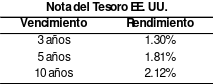
\includegraphics[width=0.3\textwidth]{image/tabla1.png}

	\tiny Fuente: Reserva Federal.
\end{center}
Con fines comparativos también se obtuvo la ratio de Sharpe para el S\&P 500 en el mismo período.

\begin{center}
    Tabla 2\\
    Ratio de Sharpe para índice S\&P 500\\

    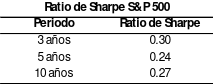
\includegraphics[width=0.3\textwidth]{image/tabla2.png}

	\tiny Fuente: Bloomberg, elaboración propia.
\end{center}


    \item Selección de Fondos Cotizados y Fondos Mutuales equivalentes: Se identificó el activo equivalente al recomendado, utilizando el índice replicado como referencia. Esto permitió determinar qué tipo de estrategias resulta más atractiva para cada inversor, de acuerdo con su perfil de riesgo y horizonte de inversión.

    \item Cálculo de Desempeño y Ratio de Sharpe de portafolios equivalentes: Se utilizó la herramienta de Backtesting mediante el portal Portfolio Visualizer para obtener los retornos de cada portafolio, y de su equivalente, a 3, 5 y 10 años. Se obtuvo el retorno anualizado, y el total, de los portafolios, así como sus respectivas ratios de Sharpe. Se supuso la reinversión de dividendos pagados, así como los costos de manejo de los activos. Se consideró al ratio de Sharpe como la métrica más adecuada para determinar la estrategia más conveniente de acuerdo al perfil y horizonte de inversión.
\end{enumerate}

\section{Resultados}
Tras la selección de las carteras y de los bancos, fue posible construir las fronteras eficientes para cada cartera y plazo estudiado, bajo los supuestos que fueron descritos anteriormente. Todas las fronteras elaboradas, junto con los portafolios y sus desempeños, se encuentran desglosados en los anexos del presente trabajo. 

Debajo se procederá con el análisis de los resultados más destacados del presente trabajo. En ellos existen algunas consideraciones previas. 

En principio, para cada banco, se espera que a medida que aumente el riesgo observado de la cartera, así lo haga su rendimiento registrado. De forma similar, se espera que a medida que el plazo estudiado aumente, así también lo haga la dispersión del desempeño ofrecido por las carteras con respecto al resultado óptimo hallado. 

Si bien el primer punto, exceptuando casos puntuales, se cumple de forma consistente, la segunda consideración fue menos certera, una vez que se obtuvieron los resultados.

A partir de este punto, se procederá con el análisis de los resultados obtenidos.

\subsection{Vanguard}
Para las carteras de Vanguard, tanto para 2014 como 2022, toda la selección de activos consiste en ETFs del banco. En total utilizaron 4 fondos cotizados, dos compuestos de acciones y otros dos de renta fija. Para cada caso, uno consiste en activos de EE. UU. (VTI y BND) y el otro de activos extranjeros (VXUS y BNDX). 

El primer aspecto para destacar en el rendimiento y ubicación de las carteras es que para todos los casos las carteras recomendadas en 2014 tuvieron un rendimiento mayor a aquellas recomendadas en 2022, sin excepción. 

Un segundo factor inmediato para destacar es el hecho de que para los portafolios en los extremos (100\% renta fija y 100\% renta variable), los portafolios recomendados se encuentran ubicados en la frontera eficiente, salvo para el caso a 10 años de 100\% renta variable, donde se encuentra la dispersión más alta de toda la muestra de Vanguard.

Por otro lado, tanto para 2014 como para 2022 se repite un patrón en cuanto a la dispersión observada entre los portafolios recomendados y el escenario sobre la frontera. Para todos los casos, salvo las excepciones mencionadas, la dispersión es creciente a medida que la renta fija es sustituida por renta variable. De igual manera, en cada caso se observa que la dispersión a 5 años es la inferior en cada cartera con respecto a los otros plazos observados.

\begin{center}
    Tabla 3.\\
    Rendimientos portafolios Vanguard y diferencia con óptimo 2014\\
    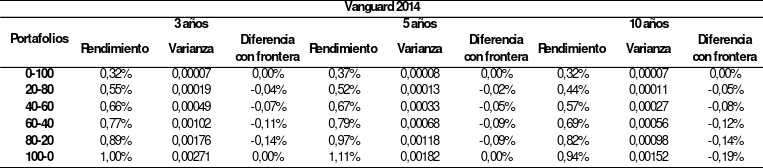
\includegraphics[width=0.8\textwidth]{image/tabla3.png}

    \tiny Fuente: Bloomberg, elaboración propia.
\end{center}

\begin{center}
    Gráfico 1\\

    Diferencia con respecto a portafolio óptimo para Vanguard en 2014\\

	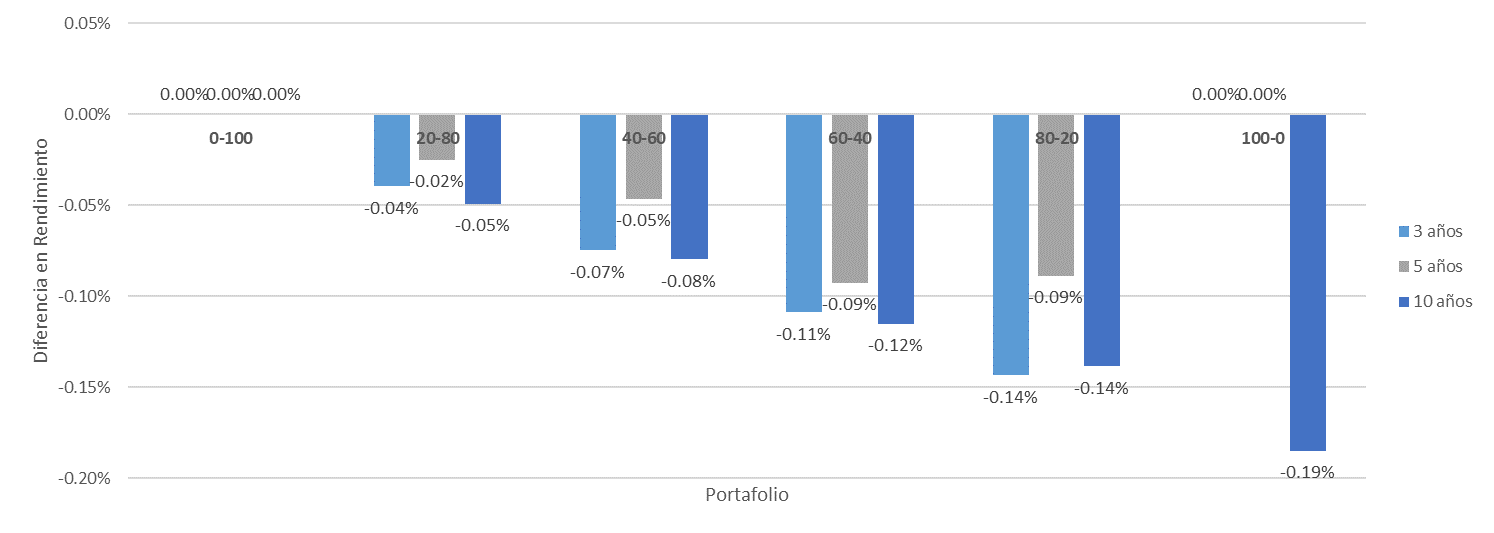
\includegraphics[width=0.9\textwidth]{image/imagen1.png}

	\tiny Fuente: Bloomberg, elaboración propia.
\end{center}

\begin{center}
    Tabla 4\\
    Rendimiento de portafolios Vanguard y diferencia con óptimo 2022\\

    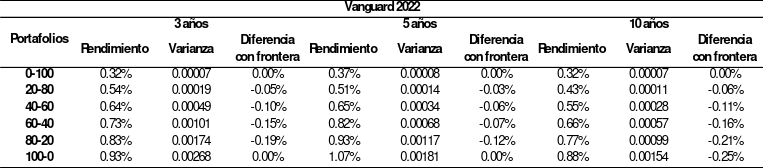
\includegraphics[width=0.8\textwidth]{image/tabla4.png}

    \tiny Fuente: Bloomberg, elaboración propia.
\end{center}

\begin{center}
    Gráfica 2\\
    Diferencia con respecto a portafolio óptimo para Vanguard en 2022\\

    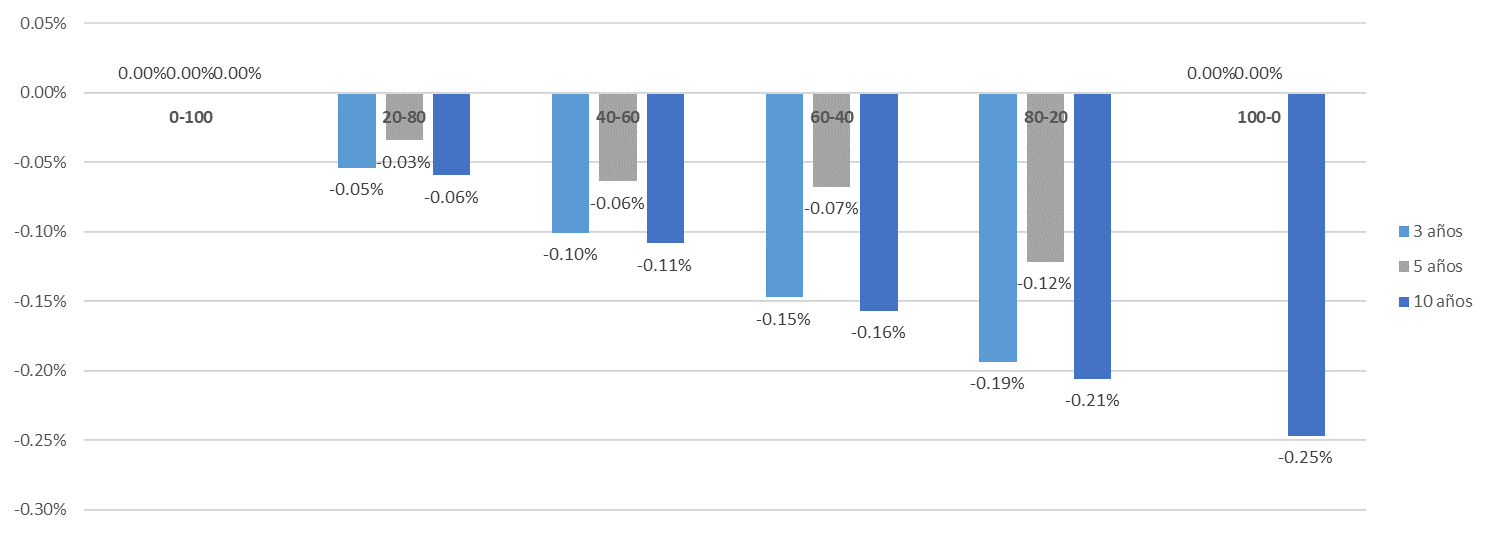
\includegraphics[width=0.9\textwidth]{image/imagen2.png}

    \tiny Fuente: Bloomberg, elaboración propia.
\end{center}

C acertado afirmar que su adición ofrece un retorno ajustado por riesgo mejor que el portafolio más conservador ofrecido por Vanguard. A partir de allí, la medida de Sharpe decrece a medida que la renta variable sustituye el peso de los bonos en cada cartera. Esta tendencia se observa en todos los plazos, tanto para las carteras recomendadas como para aquellas ubicadas en la frontera óptima. 
Por último, cuando se comparan las medidas de Sharpe de los portafolios ante la mostrada por el S\&P 500 en los mismos períodos se observa que, en general, las primeras 2 carteras recomendadas mejoran al índice de mercado. Sin embargo, a partir del punto donde la renta variable comienza a tener una participación mayoritaria en la cartera esta tendencia se revierte. Esto no sucede de manera similar en el caso de las carteras sugeridas por la frontera eficiente, donde a excepción de algunos casos, todos los portafolios ofrecen una medida de Sharpe superior a la del mercado. Especialmente a medida que el horizonte de tiempo es mayor. 

\begin{center}
    Tabla 5\\
    Ratio de Sharpe para portafolios Vanguard (2014) y diferencia con óptimo.\\

	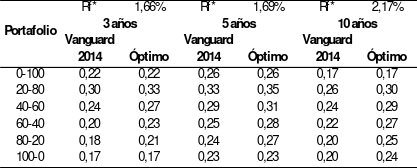
\includegraphics[width=0.5\textwidth]{image/tabla5.png}

	\tiny Fuente: Bloomberg, elaboración propia.
\end{center}

\newpage
\begin{center}
    Tabla 6\\
    Ratio de Sharpe para portafolios Vanguard (2022) y diferencia con óptimo.\\

    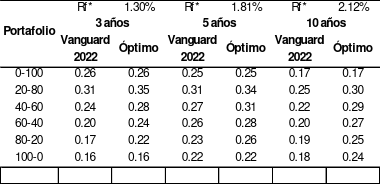
\includegraphics[width=0.5\textwidth]{image/tabla6.png}

    \tiny Fuente: Bloomberg, elaboración propia.
\end{center}

\subsection{Fidelity}
Para el caso de Fidelity, tanto en 2014 como 2022, las carteras se encontraron compuestas por fondos mutuales en su totalidad. Todos, con la excepción de (FBNDX), carecen de costos de entrada o salida. 
Una diferencia notable entre los dos años de referencia se encuentra en que en las carteras de 2014 se utilizaron en total 4 activos, mientras que en las recomendadas en 2022 se utilizaron 15 activos. 
La composición de las carteras varía de acuerdo con el riesgo. Sin embargo, todas poseen bonos y acciones, sin activos de inversión alternativa. Estas poseen exposición tanto a mercado local (EE. UU.), como a mercados internacionales desarrollados y emergentes. 
Para las carteras recomendadas en 2014 se denota una tendencia clara en cuanto a la dispersión con respecto al portafolio óptimo para cada combinación de activos. En cada portafolio la dispersión aumenta a medida que el plazo de tiempo observado es mayor. Sin embargo, un aspecto destacable es el hecho de que para el portafolio más agresivo todos los períodos se encuentran ubicados en la frontera eficiente, luego de contabilizar los costos de manejo de la cartera. Otro factor destacable es el hecho de que, exceptuando el portafolio a 10 años de crecimiento, todas las carteras se encuentran a una distancia similar al óptimo para cada nivel de riesgo. 
Por su parte, las carteras ajustadas en 2022 presentan una tendencia opuesta a las de sus pares de 6 años atrás. Esto es, a medida que el plazo observado aumenta, la distancia con respecto a la frontera eficiente disminuye. Con la excepción de los dos portafolios en los extremos de riesgo, esta tendencia se cumple en cada caso. Si es destacable el hecho de que, contrario a lo sucedido para las carteras de 2014, a medida que se aumenta el riesgo de la cartera la distancia con respecto al óptimo también aumentó.

\begin{center}
	Tabla 7\\
	Rendimientos portafolios Fidelity y diferencia con óptimo 2014\\

	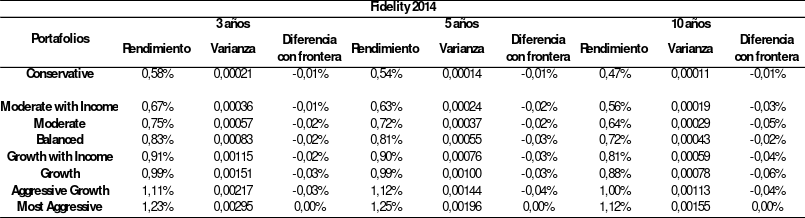
\includegraphics[width=0.8\textwidth]{image/tabla7.png}

	\tiny Fuente: Bloomberg, elaboración propia.
\end{center}
\newpage
\begin{center}
	Gráfico 3\\
	Diferencia con respecto a portafolio óptimo para Fidelity en 2014\\

	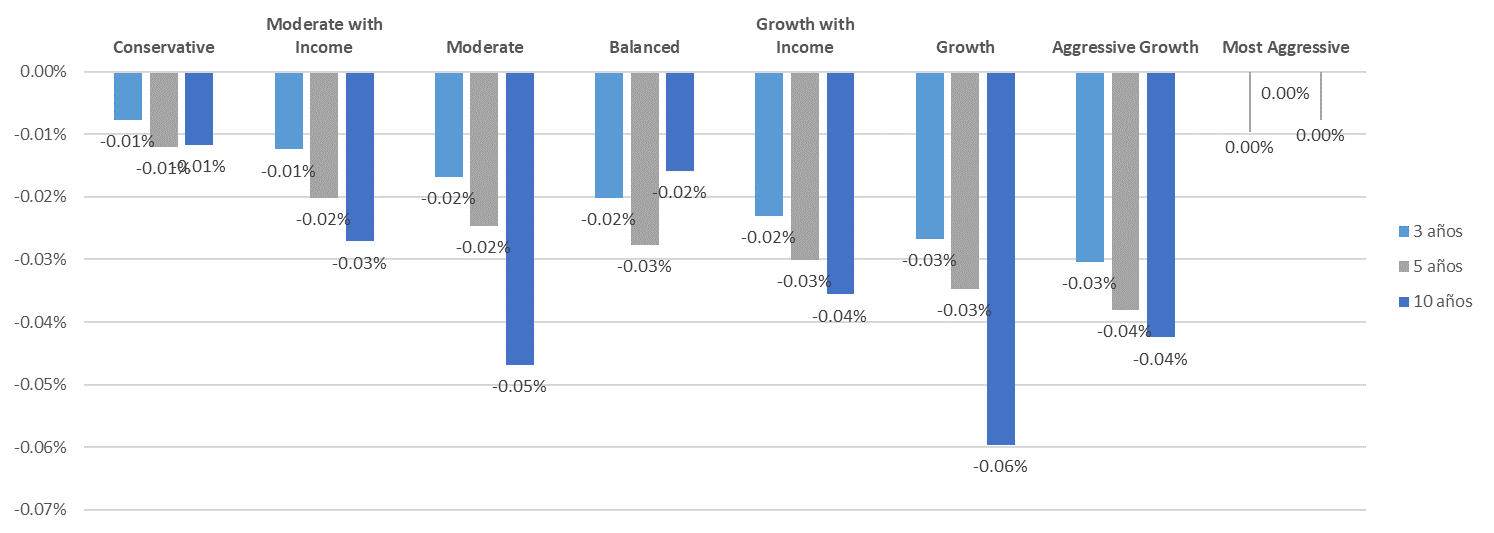
\includegraphics[width=0.9\textwidth]{image/imagen3.png}

	\tiny Fuente: Bloomberg, elaboración propia.
\end{center}

\begin{center}
	Tabla 8\\
	Rendimientos portafolios Fidelity y diferencia con óptimo 2022\\

	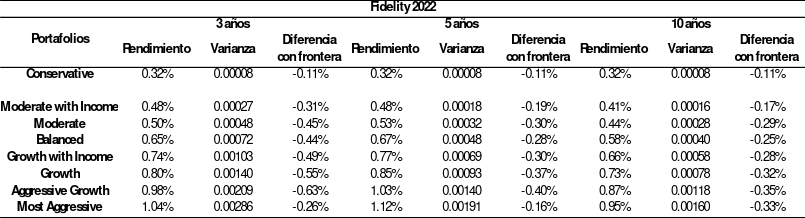
\includegraphics[width=0.8\textwidth]{image/tabla8.png}

	\tiny Fuente: Bloomberg, elaboración propia.
\end{center}

\begin{center}
	Gráfico 4\\
	Diferencia con respecto a portafolio óptimo para Fidelity en 2022\\

	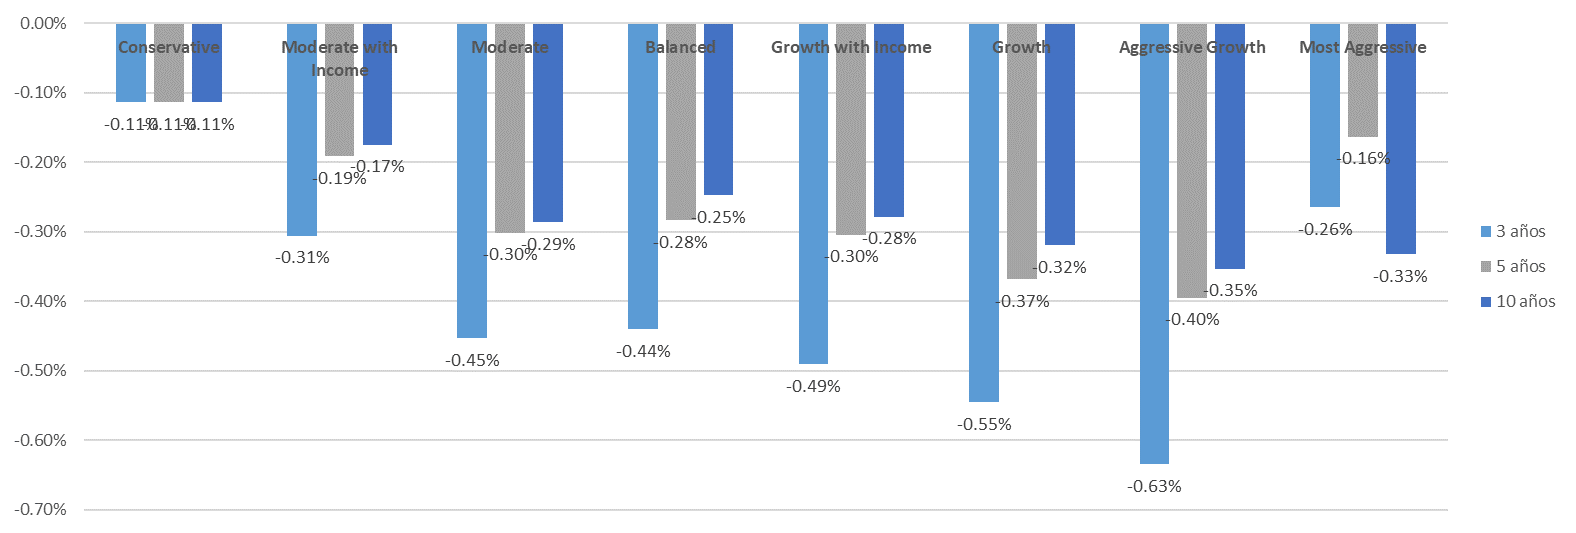
\includegraphics[width=0.9\textwidth]{image/imagen4.png}

	\tiny Fuente: Bloomberg, elaboración propia.
\end{center}

Cuando se observa el desempeño, ajustado por el riesgo, de cada cartera se destacan varios detalles. En principio, para las carteras de 2014, se observa que, sin excepción, la medida de Sharpe decrece mientras se aumenta el riesgo de estas. Esto se repite tanto para las carteras recomendadas como para las óptimas. 

Ahora bien, cuando se compara contra el S\&P 500, los portafolios a 5 años de 2014 son los únicos es tomar un valor aproximado al de mercado. El resto de perfiles y horizontes muestra un rezago considerable en comparación al mercado. Destaca que esto no sucede con los portafolios óptimos estimados para 2014. 

Lo anterior se replica en las carteras ofrecidas en 2022 difieren en lo anterior. 
Por último, y similar a lo observado en el caso de Vanguard, todas las carteras recomendadas en 2014 superan de manera considerable a sus pares de 2022, con una diferencia en promedio de 0,17\% mensual en los rendimientos ofrecidos.

\begin{center}
	Tabla 9\\
	Ratio de Sharpe para portafolios Fidelity (2014) y diferencia con óptimo.\\

	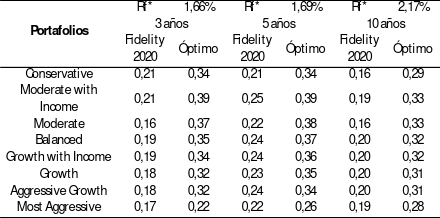
\includegraphics[width=0.45\textwidth]{image/tabla9.png}

	\tiny Fuente: Bloomberg, elaboración propia.
\end{center}

\begin{center}
	Tabla 10\\
	Ratio de Sharpe para portafolios Fidelity (2022) y diferencia con óptimo.\\

	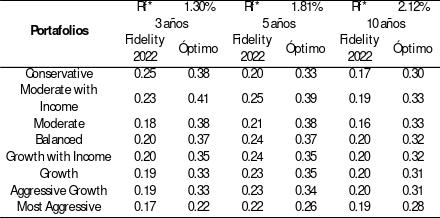
\includegraphics[width=0.45\textwidth]{image/tabla10.png}

	\tiny Fuente: Bloomberg, elaboración propia.
\end{center}

Observando los resultados, parece existir evidencia considerable para argumentar que los cambios, y aumento de activos ofrecidos, en los portafolios de 2022 no fueron justificados en su rendimiento.

\subsection{Comparación de tipos de activos y estrategias. Fondos Mutuales y Fondos Cotizados (ETFs) }

Adicional a los resultados hallados mediante la elaboración de las fronteras eficientes, se buscó estimar la efectividad de las estrategias utilizadas por una selección de tres bancos. La muestra se limitó a tres bancos dada la especificación de las carteras ofrecidas por estos. Fidelity utilizó únicamente fondos mutuales, mientras que Vanguard solo seleccionó fondos cotizados. Esto permitió buscar pares similares para establecer carteras opuestas y determinar que escenario le podría ser más rentable a un inversor con cada perfil y horizonte. 

Entendiendo que la similitud de índices de referencia puede generar ciertas complejidades al momento de comparar los tipos de activos, especialmente conociendo que mientras un ETF pasivo busca replicar el índice, el fondo mutual activo suele tratar de generar alfa partiendo de la referencia, se utilizó la ratio de Sharpe como medida definitoria para determinar que selección de cartera puede ser más conveniente ajustando por desempeño y riesgo. 

 Con lo anterior establecido, es posible notar que, salvo para el caso de Fidelity, los resultados son consistentes en todos los horizontes de inversión, con algunas excepciones.

 Para el caso de Vanguard, donde ofrecen carteras con 4 ETFs, parece ser la opción más recomendable. Exceptuando los casos más conservadores para 5 y 10 años, el resto de los escenarios son dominados por la estrategia pasiva de uso de fondos cotizados.

 \begin{center}
     Tabla 11\\
     Activo con mejor ratio de Sharpe por horizonte y perfil de riesgo para Vanguard\\

     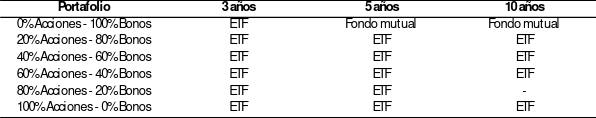
\includegraphics[width=0.6\textwidth]{image/tabla11.png}

     \tiny Fuente: Bloomberg, elaboración propia.
\end{center}

El caso donde se evidenció una mayor dispersión en los resultados fue para las carteras de Fidelity, las cuales se encuentran conformadas por fondos mutuales en su totalidad. Para su caso, en horizontes de 3 años la selección de una estrategia más activa resultó más atractiva. Mientras que, para plazos intermedios, a medida que el riesgo aumentó, la opción pasiva resultó más eficiente. Por último, para plazos largos, con la excepción de los dos casos más agresivos, donde los resultados fueron similares para cada estrategia, el uso de fondos mutuales resultó, en su mayoría, la estrategia ganadora.

\begin{center}
	Tabla 12\\
	Activo con mejor ratio de Sharpe por horizonte y perfil de riesgo para Fidelity\\

	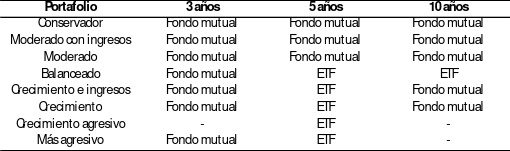
\includegraphics[width=0.5\textwidth]{image/tabla12.png}

	\tiny Fuente: Bloomberg, elaboración propia.
\end{center}

En vista de los resultados, es posible afirmar que tanto Fidelity como Vanguard poseen carteras que, al menos en la selección del tipo de activos, parecen ser las más adecuadas para la mayoría de los perfiles estudiados.

\section{Conclusiones}
El presente trabajo se fundamentó en las carteras ofrecidas por los principales bancos de inversión en EE. UU. a sus clientes, de acuerdo a los perfiles de riesgo de cada inversor. Mediante estas su buscó determinar si los perfiles ofrecidos correspondían al riesgo ofrecido, así como si las carteras eran óptimas. Para ello, se desarrolló una frontera eficiente, para cada cartera, en horizontes de 3, 5 y 10 años. Mediante éstas fue posible determinar qué tan alejados se encontraron los portafolios recomendados del punto de mayor eficiencia, dados los activos utilizados. Si bien los resultados variaron de forma considerable para cada banco, sí existió una tendencia general relacionada al nivel de riesgo ofrecido. A medida que el riesgo de las carteras aumentó, así lo hizo su dispersión con respecto al óptimo hallado en las fronteras estimadas. 

Así mismo, otro factor en común en el caso de los dos bancos (Fidelity y Vanguard), para los cuales fue posible realizar una comparación de las carteras de los años 2014 y 2022, fue que las carteras actualizadas en 2022 no resultaron ser más eficientes ni ofrecieron un mayor desempeño que aquellas ofrecidas en 2014. Estos resultados fueron consistentes para todos los periodos evaluados entre 2012 y 2022.

Otro aspecto de los resultados hallados fue la consistencia en las dispersiones, con respecto a la frontera, a través de los horizontes evaluados. Para cada plazo estudiado, salvo ligeras excepciones, las dispersiones fueron mayores para plazos largos, tanto para perfiles conservadores como agresivos. 

En relación al desempeño de las carteras, las cuales están sustentadas en criterios de riesgo y diversificación, se notó que, salvo contadas excepciones, solo los portafolios moderados y conservadores ofrecieron desempeños superiores al S\&P 500, una vez se ajustó por riesgo. A medida que el riesgo de las carteras aumentó, la medida de Sharpe no justificó el riesgo adicional tomado en los portafolios, una vez comparado con el índice de mercado. Para el caso específico de Fidelity, con la excepción de los portafolios a plazos medios de 2014, casi todos fueron inferiores al mercado. Ahora bien, con respecto a lo anterior, también fue hallado que los pares eficientes de los portafolios ofrecidos, si bien mantenían resultados similares, mostraron un desempeño mejor al mercado incluso en carteras moderadamente agresivas o de crecimiento.  

En función a los perfiles de riesgo evaluados todos los bancos mostraron congruencia en los portafolios recomendados, de acuerdo al riesgo ofrecido. Esto es, evaluando el portafolio de mínima varianza para cada cartera, a medida que se aumentó el riesgo, la cartera ofrecida mostró una mayor distancia con respecto al punto de mínima varianza, y al portafolio que le precedía en criterios de riesgo. 

En último lugar, buscando establecer criterios de selección de activos más adecuados, se buscó comparar carteras de acuerdo al tipo de vehículo de inversión ofrecido. Usando de muestra a 2 bancos, de los cuales sus carteras se encontraron conformadas únicamente por un tipo de activo, se estableció una comparación entre Fondos Mutuales, como proxy de manejo activo de inversiones, y Fondos Cotizados (ETFs), como proxy de inversión pasiva. 

Usando las carteras de Fidelity y Vanguard, se determinaron portafolios equivalentes, utilizando un vehículo de inversión opuesto al ofrecido por la cartera, utilizando el índice replicado por el activo como modelo para hallar la equivalencia de los activos, y se realizó una comparación por perfil de riesgo y horizontes de tiempo a 3, 4 y 5 años, midiendo el desempeño de cada cartera. Se utilizó la medida de Sharpe como criterio de decisión.  Las carteras mostraron unos resultados mixtos. Para Vanguard, los portafolios compuestos por ETFs obtuvieron un mejor ratio Sharpe que su equivalente en fondos mutuales. Sin embargo, para Fidelity se observa como a 3 y 10 años los fondos mutuales tienen mejor desempeño que sus equivalentes en ETFs, pero a 5 años en los portafolios más expuestos a la renta variables los ETFs consiguen un mejor ratio que los fondos mutuales. Es de destacar que, tanto Fidelity como Vanguard, al menos en lo que a selección de tipo de activos se refiere, parecen encontrarse ofreciendo las mejores opciones, salvo excepciones. 

En lo observado para ambas instituciones es posible afirmar dos cuestiones. En primer lugar, los resultados de los portafolios modificados en 2022 no resultaron en mejoras para sus clientes, al menos en término de desempeño y riesgo. En segundo lugar, ambas instituciones si parecen justificar el uso de las estrategias seleccionadas para cada perfil de riesgo, en términos generales, aunque no absolutos. Algo que se debe destacar es que, contraria a la hipótesis de esta investigación, el uso de estrategias activas fue más justificable en perfiles más conservadores.

Como cierre resulta útil comentar algunas limitantes del presente trabado y recomendaciones para futuros trabajos. 

La investigación actual abarca un margen amplio de temas que ofrecen un espacio considerable para futuros trabajos. En primer lugar, habiendo considerado los costos de manejo de todos los activos utilizados, sí es recomendable, para futuros estudios, agregar los costos de corretaje, especialmente para los Fondos Mutuales, los cuáles pueden ser determinantes en el análisis comparativo con respecto a los fondos cotizados. 

Por su parte, para el presente trabajo, se consideraron fondos cotizados de manejo pasivo, dado que estos son los ofrecidos por los bancos estudiados. Sin embargo, en el presente, cada vez son más populares los fondos cotizados de manejo activo. Si bien no han estado en el mercado un tiempo suficiente como para evaluar sus resultados de manera consistente, sí se considera como un factor a tomar en cuenta en futuros estudios comparativos. 

Adicionalmente, por limitaciones de espacio y recursos, el estudio de carteras se limitó a las ofrecidas en 2014 y 2022 por dos instituciones. Parece útil ampliar la muestra estudiada en estudios posteriores.

\newpage

\begin{center}
    \textbf{ANEXO (v. reducida)}
\end{center}

\begin{center}
    Gráfica 5.\\
    Frontera eficiente a 3 años para portafolio 80-20 para Vanguard.\\

    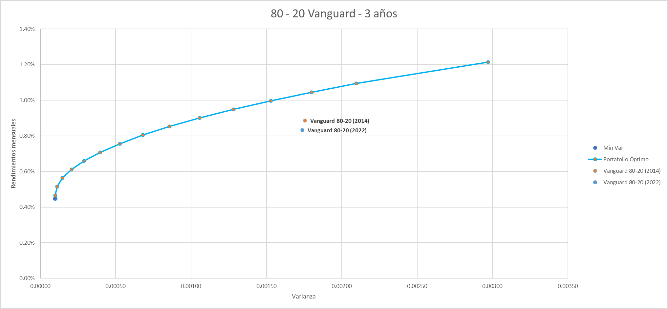
\includegraphics[scale=1.5]{image/imagen5.png}

\end{center}

\begin{center}
    Gráfica 5.\\
    Frontera eficiente a 3 años para portafolio 80-20 para Vanguard.\\

    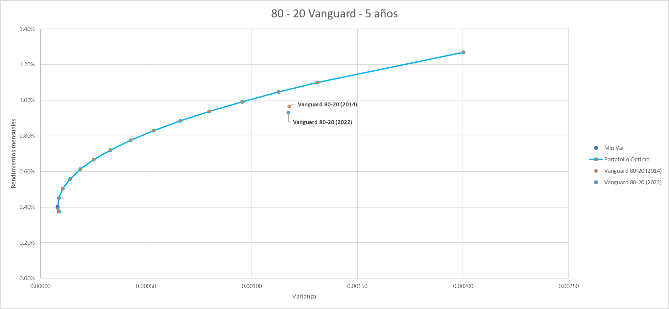
\includegraphics[scale=1.5]{image/imagen6.png}

\end{center}

\begin{center}
    Gráfica 5.\\
    Frontera eficiente a 3 años para portafolio 80-20 para Vanguard.\\

    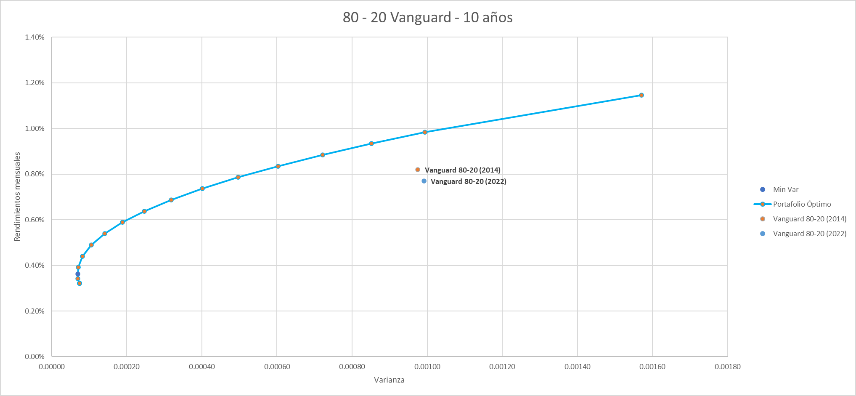
\includegraphics[scale=1.2]{image/imagen7.png}

\end{center}

\newpage

\begin{center}
    Tabla 13.\\
    Resultados de Backtesting para cada perfil y horizonte de acuerdo con el activo utilizado para Fidelity\\

    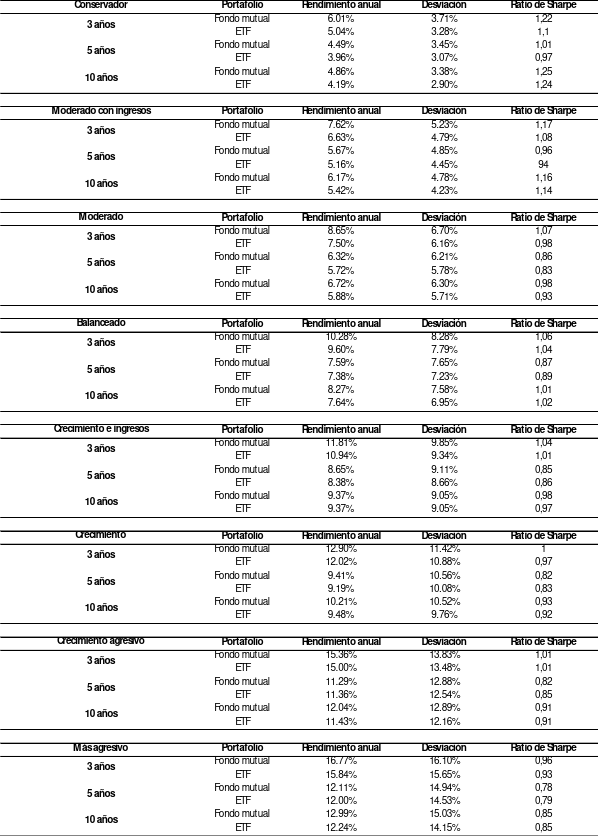
\includegraphics[scale=.7]{image/tabla13.png}

    \tiny Fuente: Bloomberg y Portafolios Visualizer, elaboración propia.

\end{center}




\begin{comment}

\section{Objetivo(s)}
Hallar las proporciones representadas por diversos instrumentos financieros en las
carteras recomendadas por los principales bancos de inversión a nivel internacional a sus clientes (en
función de su perfil de riesgo), y determinar cuál ha sido el desempeño de esos portafolios en los
últimos 3, 5 y 10 años. Además, se analizará si el desempeño de las carteras muestra divergencias
considerando el tipo de estrategia seguida (activa o pasiva).

\section{Problema o problema central} 
¿Cuál ha sido el desempeño histórico de las carteras recomendadas
por los principales bancos de inversión, ajustado por criterios de riesgo y tipo de estrategia (activa o
pasiva)? ¿Ha sido este desempeño congruente con el estilo y riesgo asumidos?

\section{Bases teóricas} 
\cite{fama1970}, establece una teoría en la que describe que el precio actual de
un activo refleja toda la información disponible que exista acerca del mismo, sea la información:
histórica, pública y/o privada. En base a ello, y considerando la eficiencia de los mercados
desarrollados, los instrumentos de inversión pasiva han mostrado un crecimiento en detrimento de
otros instrumentos activamente gerenciados, tales como fondos mutuales, dado el mejor desempeño
histórico que ha exhibido las estrategias pasivas.

Así, por ejemplo, \cite{Chan1999} consiguen que solo una baja proporción de los
fondos activamente gerenciados logra superar, de forma persistente, al desempeño de los índices de
referencia pasivos del mercado. \cite{Pastor2020} hallan que durante la crisis de la COVID-19 el
flujo de fondos hacia vehículos de inversión activa ha disminuido, aunado a un desempeño inferior en
relación a los índices de referencia y fondos de inversión pasiva. Todo ello va de la mano con la teoría
moderna de portafolios, desarrollada por \cite{Markowitz1952}, la cual establece un modelo que consiste
en ubicar una cartera de inversión óptima, ajustada por el riesgo, mediante la elección de los activos
adecuados que compongan dicha cartera.

\section{Hipótesis} 
La inversión ha sido una práctica que con los años se ha vuelto cada vez más popular. En
sus comienzos era solo aplicada en países muy específicos, pero se ha globalizado y hoy en día es
conocida y desarrollada en una gran variedad de países. 

En el pasado existían muchas limitantes a la hora de invertir en el mercado de valores. Era necesario
tener acceso a una cuenta de jubilación proporcionada por un empleador de una compañía, o poseer
los fondos y el conocimiento suficiente para poder abrir una cuenta de inversión no patrocinada por
un empleador.

Con el pasar de los años estas limitantes se han ido mitigando y el tener acceso a una cuenta de
inversión se ha vuelto cada vez más sencillo. Existen múltiples herramientas financieras que le
permiten a los inversionistas adquirir participación en una empresa sin hacer uso de una gran cantidad
de fondos. Además, existen muchas compañías que permiten abrir cuentas de inversión a nivel
mundial desde plataformas virtuales, múltiples cursos de inversión e información de fácil acceso a
través del Internet.

Sin embargo, a pesar de la facilidad que existe para adquirir información hoy en día, muchos de los
nuevos inversionistas no cuentan con los conocimientos necesarios para poder manejar sus
inversiones de la forma más eficiente posible o guiarlas de acuerdo con sus necesidades. Lo anterior
se debe a que, en su mayoría, estas personas desconocen cuáles son sus metas financieras y sus
limitantes a la hora de invertir, por lo cual no utilizan estrategias de inversión que vayan de la mano
con sus expectativas.

Por esto último, la industria financiera, mediante bancos de inversión, ofrece asesorías de inversión
hacia clientes, especialmente con ciertos requerimientos mínimos de patrimonio. De forma usual,
ante la mayor demanda de este tipo de servicios, muchos bancos optan por ofrecer portafolios
estandarizados bajo ciertos perfiles de riesgo.

En base a lo anterior, las instituciones financieras recomiendan sus carteras a los inversores que
encajen en cada perfil ofrecido. Si bien esta práctica responde a una necesidad, podría estar dejando
de lado ciertas oportunidades de mejora. Esta investigación se enfoca en indagar sobre este tópico y
poder así determinar si los portafolios ofrecidos a los inversionistas se ajustan a los perfiles de riesgo
establecidos, y si éstos pueden ser considerados óptimos, o presentan un espacio de mejora en el
desempeño. De igual forma, se busca establecer si la estrategia ofrecida resulta ser la más beneficiosa
por perfil y horizonte de tiempo,

\section{Método o plan de investigación} 
Se utilizará la base de datos de Bloomberg para obtener el
rendimiento y el riesgo de los índices de precios de acciones y bonos (por ejemplo, S\&P 500 e índices
de bonos de Barclays), así como también las composiciones de los portafolios estandarizados ofrecidos
por los principales bancos de inversión a nivel mundial (tales como Blackrock, Vanguard, Merril Lynch
y Charles Schwab) a sus clientes en función del perfil de riesgo.

Se hallará la frontera eficiente para cada período de tiempo considerado varios supuestos (ventas en
corto no permitidas y existencia de una tasa de interés libre de riesgo), y utilizando activos
tradicionales (acciones y bonos).

A continuación, se examinará si los portafolios recomendados por los bancos de inversión se ubican
en la frontera eficiente (se analizará si el rendimiento de la cartera de la frontera eficiente que tenga
la misma desviación estándar que la cartera recomendada por el banco de inversión respectivo es 
estadísticamente igual -usando varios niveles de significación estadística, - similar al análisis
desarrollado por \cite{Garay2005}. Lo anterior se hará para períodos de referencia de 3,
5, 10 años (2012-2022), evaluando si el riesgo evidenciado por las decisiones de inversión se ajustó a
sus rendimientos, mediante el uso del ratio de Sharpe.

Para establecer una comparación aproximada del rendimiento de un portafolio recomendado, por
perfil de riesgo, compuesto por un solo tipo de activos con respecto a un mismo portafolio de un tipo
de activo similar, se considerará identificar el activo equivalente al recomendado, utilizando el índice
replicado como referencia. Esto es, si la recomendación incluye únicamente fondos mutuales, se
determinará que fondos cotizados (ETFs) son equivalentes a esos fondos mutuales, y viceversa, a
modo de determinar qué tipo de estrategias resulta más atractiva para cada inversor, de acuerdo con
su perfil de riesgo y horizonte de inversión.

\section{Conclusiones y resultados} 
Se espera hallar una congruencia entre el nivel de rendimiento exhibido por las carteras de los bancos de inversión y la correspondiente a las carteras ubicadas en la frontera eficiente obtenida (con el mismo riesgo). Además, se espera que las carteras de inversión activas recomendadas por los bancos exhiban un desempeño inferior al de las carteras pasivas, ajustadas a su riesgo.

\end{comment}

% To print the credit authorship contribution details
\printcredits

\bibliographystyle{cas-model2-names}

% Loading bibliography database
\bibliography{refs}

% Biography
\bio{}
% Here goes the biography details.
\endbio



\end{document}

